
\documentclass{article}
\usepackage{mathtools}
\usepackage{graphicx}

\title{CS 571: AI}
\author{Roscoe Casita}
\date{}
\begin{document}
\maketitle
\section{A survey, application, background and proposal for AI applied to battery chemistry}

A common saying in AI is ``All models are broken; some are useful''; thus AI is the search for useful models. The physical chemistry domain maps to this concept perfectly as there are multi-scale level of models which are all broken at the wrong scale yet still useful at the right scale. This survey reviews computationally complex problems in chemistry; an applied AI technique used to solve one; direction for future work; and a proposal. The following are considered: predicting new materials and chemical compounds, predicting laboratory results from training data, analyzing and solving all possible reactions for a given set of compounds, exploring the classification of reactions, and proposing future directions of research based on related works. \\

Fundamentally all problems have a representation and encoding of the solution. Optimizations and gains in efficiency exploit symmetries found in the representation model which lead to either a smaller encoding or faster convergence upon the encoding. Building AI space representations requires an intimate understanding of the specific problem at hand to build an appropriate abstraction and approximation.  As each representation varies drastically in its ability to model problems correctly; an optimal mapping of representation to problem determines if the solution is tractable or not. Selecting the wrong representation is not simply a performance issue, but guarantees that there is either no encoding of the solution or the time to find the encoding is exponential.\\

Search trees, constraint satisfaction, decision policy, and iterative learning are some of the weapons to choose from as an AI systems designer. The selected problem of enumerating all reactions will demonstrate effective search tree modeling. Results of the search will be examined as a model that will be used in further research. Future work will highlight filtering reactions via features extracted using constraint satisfaction. The techniques used for predicting molecules and laboratory results breach the scope AI into machine learning when artificial neural networks are used.
\newpage
\section{Predicting new molecules and compounds}
AI has been used to solve computationally complex problems in the organic biomedical field with tangible results and benefits.  There are several crowning achievements that have resulted in experimental research drugs, improved organic chemical manufacturing, and designs for new polymer materials. In all the examples presented, AI is used to create a relaxed model that can extrapolate a prediction modes given enough sample data. AI is used to solve a particular subproblem in chemistry such as predicting the stability of new organic carbon ring compounds or predicting the optimal laboratory conditions to extract the maximal yield from a reaction. Any system that seeks to apply AI to problems in chemistry needs to isolate and restrict the abstract model to the particular area otherwise the noise and error grows exponentially. \\

Designing new physical materials such as stronger metal alloys, plastics resistant to corrosion, drugs to target cancer, or energy dense electrolytic solutions requires extensive background knowledge in the precise area. During the last 30 to 50 years significant advances in designing new materials have come from applied techniques of artificial intelligence. Fundamentally these problems originate from the multitudes of micro/macro models in chemistry. Quantum mechanics describes the exact properties of atoms at a micro scale in both size and time that can not be computed at the macro scale. Molecular dynamics predicts properties but at a macro scale resulting in the loss of resolution on the micro scale. The properties of materials can be both described and measured easily; predicting these values based on quantum simulation is computationally difficult without relaxations in the model to allow for approximations. DFT made significant progress towards approximate models at larger micro scales, but was still not able to model the macro scale. Simulations of rudimentary physics describe the expected behavior at the macro level but are unable to model features at the micro level. Recently research has been able to extract and predict macroscale properties from microscale models. The extracted correlation between macro and micro properties stored in the representation, models the appropriate mathematical actions to relax the exact calculations to the scale of the micro systems. \cite{HEURISTIC}  Features, properties, and environmental controls were found and exploited to generate new materials and accurately predict their properties before performing laboratory experiments.  \cite{PROPERTIES} \\ 

Consider the state space of representing all molecules composed of a number of atoms from a set of elements. Each element has a given number of valence electrons that can form bonds with the other elements in the molecule. As the bonds can potentially be between any of the atom's valence electrons; the number of possible configurations for a single molecule grows faster than exponentially in the number of valence electrons for the given atom. \\

$${ValenceElectrons} ^ {Atoms ^ {ValenceElectrons^{Atoms}}}$$ 

\newpage
\section{Predicting accurate laboratory results}

Reactions are governed by a multitude of factors from heat, pressure, voltage, to molarity, velocity, and shape of the container. These factors can lead to predicting inaccurate results when a chemist with domain knowledge would predict the correct result. Researchers have used these control variables as the training data to control the desired outcome of a reaction.\cite{NICKEL}\cite{TENSOR}  Thus the AI was used to learn and determine the optimal parameters to control the environment to produce the desired result from the chemical reaction. Not only is there evidence that the AI techniques produce excellent results, but there is proof that the machine learned neural network could generalize information into a model that can be extracted to determine new undiscovered fundamental properties of physics and chemistry. \\

A prime example of the important difference between calculated density functional theory values and experimental is the simple $H_2O + O_2 = H_2O$ reaction which has a calculated energy of $-8.3eV$ vs. the experimental of $-5.9eV$.  The advances that density functional theory promised to deliver have fallen short of bridging the difference between calculated models and laboratory results. DFT is highly useful in the organic and biomedical field as the characteristics of large macroscopic molecules fit the DFT model well. The DFT model is arguably better then the full solution to Schr\"{o}dinger equation, since it provides an approximate result at the macro scale. The Materials Science Project initiative has been established to solve this complex problem directly as the multitudes of correct models do not match laboratory results. \\

The problem is that DFT does not model the microscale features at the level needed for physical electronic chemistry. Thus DFT models produced predictions which varied $\pm 1eV$ from test results. As the operating range for electronic reactions is sub $\pm 0.1eV$ the models inaccuracies are unable to compensate without further enhancements to the predictive capability of the system. These differences demonstrate how the exact equation calculation fails to accurately predict real laboratory test results. These differences can be bridged by using the calculated values alongside the experimental values as training data. Extracting the conditions, controls, and components of the reaction is difficult yet rewarding; after training over these models, extraction of predicable results were achieved. \cite{SILVER} \cite{ALO} \\

Future techniques are under investigation for creating fine and course grained models which can be used in parallel with laboratory data to create training data for machine learning systems. The majority of these techniques leverage machine learning systems to build predictive models as opposed to state space exploration, utility maximization, or constraint satisfaction. Recent work by Pedram Rooshenas and David Ozog will be explored for future research in building predictive models that exploit quantum, molecular, and laboratory data as training systems. \cite{PEDRAM} \cite{DAVID}

\newpage
\section{Enumerating all reactions}
Calculating all the possible reactions from a given set of compounds is provably NP-hard. Each reaction contains product and reactant sides of the equation; all subsets of compounds appear on both sides of the equation. Thus the complexity is $2^{Compounds} * 2^{Compounds}$. The recent discovery of the null matrix technique for balancing chemical equations improves the maximal upper bound to\cite{BALANCE}: $$\dfrac{{Compounds}!}{ Elements! * (Compounds - Elements)!}$$ 

The lower maximal bounds significantly overestimate the number of reactions in practice, as the real bound is the count of eigenvectors of the compound decomposition matrix. As the number of compounds grows larger the number of unique elements does not grow beyond the periodic table. The naive matrix representation has one row for every element and one column for every compound. The problem with this representation is that the solutions are only with respect to compounds in the first N columns, where N is the number of rows. In order to find all the reactions all combinations of size N picked from the compounds must be selected with the naive technique. \\

Only the mass laws of chemistry are taken into consideration for this state space and the space is still potentially unbounded for practical consideration. The entire space of all reactions includes linear combinations of reactions such as $\{CH_4 + 2H_2 + 3O_2 = 4H_2O + CO_2\}$ which can be broken down into a combination of $\{2H_2 + O_2 = H_2O\}$ and $\{CH_4 + O_2= CO_2 + 3H_2O\}$.  As linear combinations can be composed of any scaler value in the domain of $[-\infty,\infty]$ this space must be avoided at all costs when represented as a space exploration search problem. All linear combination reactions are derived from unique reactions, thus the reduced unique reaction space is essential to extract and to create a minimal representation of the state space. Each unique reaction is the result of a row reduced echelon form eigenvalue extraction technique. Sets of compounds are  decomposed into a matrix and solved using exact rational numbers in order to guarantee accuracy. Computing exact rational numbers is computationally expensive but necessary to extract the exact mass law balanced coefficients. \\

The infinite space can be divided into 3 subspaces: ``Not a Reaction'', ``Unique Reaction'', and ``Linear Combination''. The not a reaction classification for a given set of compounds represents a sub space that needs to be explored further to find unique reactions. Unique reactions generate one and only one decomposition of mass law coefficients that balance the equation. Linear combinations are sets of compounds that contain unique reaction subsets within them. From traditional set theory, draw a circle on a piece of paper to represent the spaces. \\
\begin{center}
	
\includegraphics[scale=.5]{circle.eps}\\
\end{center}

This diagram is representative of the space division, the white space inside the circle is the ``Not a Reaction'' space, the black circle itself is the ``Unique Reaction'' space, and the gray space outside the circle is the ``Linear Combination'' space. An unresolved question is the size of the unique reaction space, if the space grows unbounded then any representation will need to be generated algorithmically to be explored, if the space does not grow unbounded then the representation can be stored in its entirety in a physical medium.\\

A compact ``Forest of Trees'' representation can be constructed as a list of nodes with indexes. The index of a node determines both the parents and the children of the given node. A ``Forest of Trees'' search system is used to construct a representation of the entire combinational space which is explorable via an algorithmically controlled depth / breadth mechanism. The ``Forest of Trees'' is traversed until a ``Unique Reaction'' is found, then traversal is correctly moved to the next possible reaction. Traversal is handled with explicit control over the depth and breadth expansion. Each leaf node represents a potential reaction composed of the path from the current tree root to the current leaf node.\\

 If the current path is not a reaction, then depth control expands the length of the search path by one. If the current path is a ``Unique Reaction'' then breadth control changes the current leaf to the next leaf with respect to the previous depth in the path through the ``Forest of Trees''. If the current path reaches the end of the forest, then the parent node advances one and the path length is shorted by one. Thus the ``Linear Combination'' reaction space is avoided as a bad game move for the exploration agent, and is never examined. \\
 
  The fringe of the search tree traversal is collected and composed into a hypergraph of all possible unique chemical reactions for a given set of compounds. Each hyperedge is a reaction with the weights representing the exact mass law balanced coefficients of the reaction. The value of each hyperedge is the arbitrarily selected feature of calculated reaction energy from the connected molecule nodes. \\

\noindent
\begin{tabular}{l | c | r}
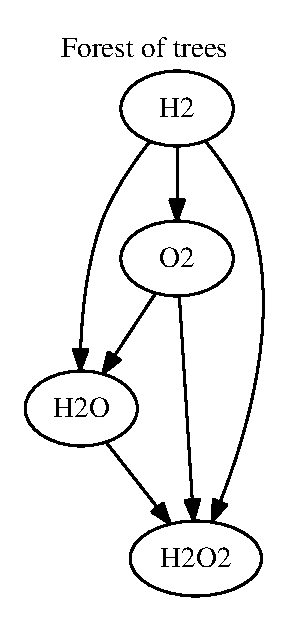
\includegraphics[width=2cm, height =5.1cm]{ForestTrees.eps}
&
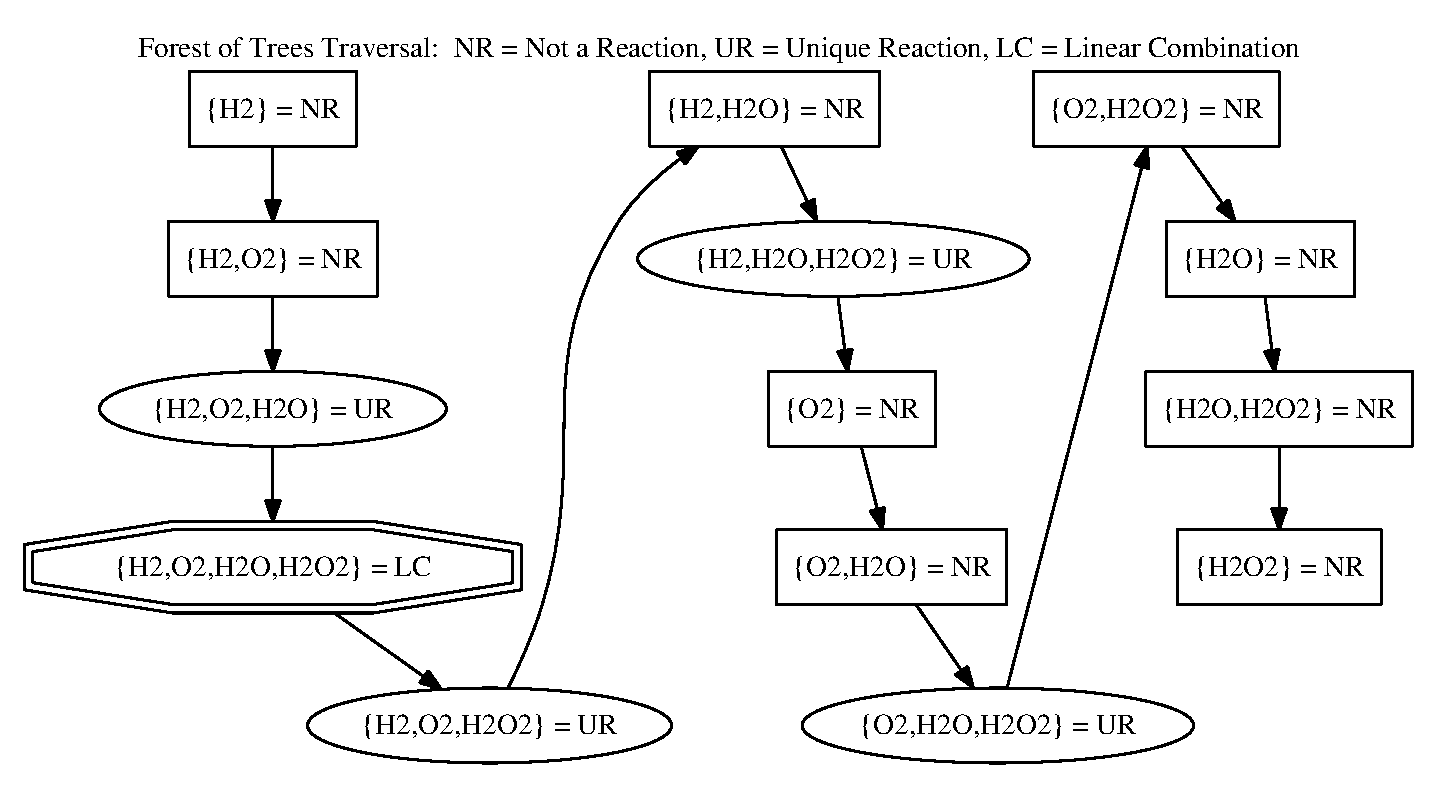
\includegraphics[width=6.5cm, height =5.1cm]{traversal.eps}
&
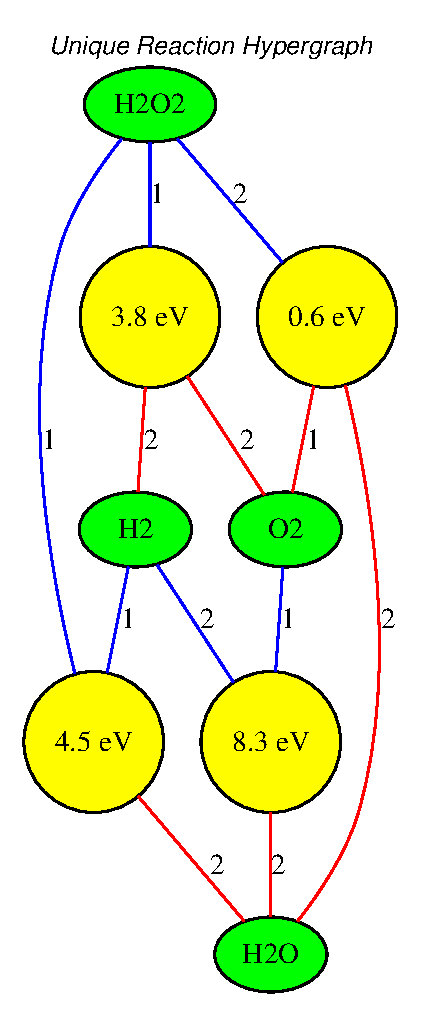
\includegraphics[width=2.5cm, height =5.1cm]{hypergraph.eps}
\\
\end{tabular}

The majority of the search space resides in the ``Linear Combination'' space as the ``Forest of Trees'' grows large. This simple algorithm based on the branch and bound / alpha-beta pruning technique is used to stop the traversal when a ``Unique Reaction" is detected.\cite{BRANCH} Eliminating the visitation to $\{H_2,O_2,H_2O,H_2O_2\}$ is the key to making this strategy tractable for solving this problem. Thus this simple technique solves the problem of building the hypergraph network of all possible mass law balanced reactions for a given set of compounds. \\

The dominating feature that affects performance for this particular search algorithm is the ordering of the ``Forest of Trees" structure.  As the number of compounds grows, the number of eigenvectors and the number of hyperedge reactions grows as well. Reaction state spaces on the order of $2^{600}$ were found to have between 10M and 100M unique reactions and thus unique eigenvectors for the particular compounds being considered. There is still an unanswered question about the maximal size of the hypergraph of all reactions as they grow, but determining if they grow unbounded has not yet been proved. The hypergraph of all possible reactions for a given set of compounds can be used as an exact model that can be learned, trained, and predicted. \\

All the possible pathways through a set of hyperedges in the hypergraph is of exceptional interest as they represent sequences of reactions either simultaneously or over time. Discharging and charging a battery are represented as a cycle of hyperedges where the cycle oscillates between at least two sets of compounds, one set for the charged state and one for the discharged. \\

Alternative pathways through the set of hyperedges that require less activation energy are characteristics of catalysts. Catalysts reduce activation energy while not directly participating in the reaction. Catalyst reactions can be represented as sequence of sub reactions where the catalyst does participate in the reaction to change the configuration of the compounds so the total pathway cost is lower. Detecting these alternative pathways is effectively a generalized search for a catalyst for a specific reaction. As an agent seeking to minimize energy costs the alternate pathway represents the optimal move in the energy state space.\\

Degenerate reaction pathways are characterized by the resultant compounds; if the compounds require significant energy or the reaction is not reversible then the pathway is characterized as degenerate. Degenerate reaction pathways can be seen in lithium ion batteries when discharging a battery with under 20\% capacity and by charging a battery with over 80\% capacity. Degenerate reaction pathways are similar to an enemy agent seeking to maximize entropy by always choosing the reaction resulting in a compound least likely to react. Thus the battery forms compounds which can no longer charge or discharge after the adverse reaction selected by the entropy opponent. \\
\newpage
\section{Extracting reaction classification and utility}
Classification of a given reaction as oxidation-reduction (redox) is important as a distinguishing feature. If there is no oxidation state change then the reaction is characterized as a participate reaction, such as liquids turning to solids.  Redox reactions are of interest as all batteries exploit these mechanics to provide electrical current. Calculating the oxidation state of each atom in a compound is exponential in the number of oxidation states for each atoms: $${OxidationStates}^{Atoms}$$ 

A reaction exhibits the redox property if the oxidation state of at least one atom in a given reaction changes. Deciding if the oxidation state changes can be reduced to a constraint satisfaction problem that can be solved with a greedy heuristic. This constraint satisfaction problem seeks to find a satisfying assignment of oxidation states to each atom in a given molecule. Oxidation states are determined by the electro negativity of the given element in the given compound. Thus an ordered list of elements sorted by electro negativity is traversed, assigning all atoms of type element to their preferred oxidation state. Elements that are less electronegative are assigned oxidation states last as a heuristic rule from chemistry. Total oxidation states for a molecule is the sum of all atoms' oxidation states and must sum to zero to maintain an overall neutral charge in the molecule. This constraint defines the conditions to assign oxidation states for each atom in a compound.\\

Determining if a reaction is redox requires that all atoms in all compounds be assigned the correct oxidation state. Given that all atoms in all compounds have the correct exact oxidation state, a perfect matching greedy algorithm can quickly determine the magnitude of oxidation state change. First, collect all the $\{atom,oxidation\}$ pairs on both sides of the reaction. For all pairs, if there is a matching $\{atom,oxidation\}$ pair on both sides then remove both pairs from both sides. The greedy algorithm continues until there are either no pairs left or there are no matching pairs. If there are no pairs left then the reaction does not exhibit the redox property. If there are pairs left, then the reaction is redox and the magnitude of oxidation state change is the absolute difference between the reactant and product sides of the reaction. \\

Thus there are multitudes of rich features that can describe the characteristics of reactions. Determining the exact set of features to extract depends upon the context of the problem being solved. Including the correct features is essential for any learning system can only extrapolate the model through the information exposed in the feature vector. Failure to include the correct feature for a given problem will result in failing to find the solution to the problem.

\newpage
\section{Features and classifications of batteries}

\subsection{Planning and background.}
The construction of an accurate simulation environment which can predict half-cell potentials, activation energies, and characterize battery performance before testing in the laboratory can reduce the costs of empirical testing by magnitudes. The disconnect between chemical composition, expected reaction physical configuration, and empirical measurements can be bridged using a series of AI and machine learning techniques to learn the real world results to build better approximate models. The databases of known material compounds is growing; by inference the hyper graph of all possible reactions is growing as well.  The perfect model for all simulations is impossible. Fundamentally there are multiple models at varying scales that describe chemistry from approximate to exact. Modeling each aspect of the features of chemical reactions leads to a complex system that must be designed upfront for future expansion as more or less detail is added and/or removed.\\

\subsection{Future battery feature learning}
AI and machine learning will be applied to learn the features and classifications of chemistry models at various levels. Here features and classifications are used to describe the various aspects of materials, reactions of those materials, batteries, and metrics of performance. Hidden features which are not discovered or named need to be accounted for in the AI model as hidden nodes which cannot be sampled or observed. The following are features of materials that are available from the materials science project database. A simple common chemical compound such as $H_2O$ can have over 20 different distinct entries representing the different phases and shapes of the material. \\

\noindent
\begin{tabular}{|c c c c|}
	\hline
	Elements & Density & Stoichiometry & Ionization energy\\
	Bond types & Symmetry group & Magnetic moment & Formation energy\\
	Oxidation states & Band Gap & Lattice parameters & Bond lengths\\
	\hline
\end{tabular}\\

The following features are selected from the sets of materials and physical constraints. Even if every feature variable domain is highly restricted the combinations grow exponentially in this example: $$O(4^N*4^R)$$
\noindent
\begin{tabular}{| c c c c|}
	\hline
	Anode material & Cathode material & Charge carrier & Charge holder \\
	Shape (mesh) & Volume & Surface & Interface layer\\ 
	\hline
\end{tabular}\\

The set of reaction features is the greatest unknown as some of the values must be derived from analysis of experimental data, such as activation energy with respect to catalysts over time. These features can currently be learned from book material and tested via inferred data. Values that cannot be directly sampled in the laboratory but only inferred after analysis of the data, will be modeled as internal variables that can still be examined.\\

\noindent
\begin{tabular}{| c c c c|}
	\hline
	Half-cell potential & Reduction potential & Catalyst & Activation Energy \\
	Electronic potential & Oxidation potential & Inhibitor & Enthalpy \\
	\hline
\end{tabular}


The next set of features is also commonly profiled with respect to batteries specifically. These features can only be sampled from complete complex systems. These features can be shown to influence the other features. Raising the temperature modifies the internal resistance which changes the amperage that affects the discharge and charge rates which raises the operating temperature... These features also vary with respect to time and charge cycles.\\

\noindent
\begin{tabular}{| c c c c|}
	\hline
	Discharge rate & Charge rate & Discharge efficiency & Charge efficiency \\
	Temperature & Voltage & Resistance & Amperage \\
	Time to charge & Time to discharge & Enthalpy & Entropy\\
	Power density & Shelf life & Charge cycles & Ambient temp \\
	\hline
\end{tabular}	




\subsection{Model building and extrapolation}
After proving that the models and simulation produce results similar to text book examples of the given features then the data gathering phase of the project is ready to proceed.  Ideally a national laboratory will already have the necessary data to draw upon so that limited numbers of actual experiments need to be performed. The specific goal would be to have a total spanning set of battery reactions that cover the viably sustainable elements which are commercially available today. Several batteries will need to be saved to validate that predicted results match real experimental results within acceptable margins of error. Any such simulation will contain multitudes of abstraction layers representing the model and encoding of parameters for optimal battery construction.  \\

\noindent
\begin{tabular}{| c c c c |}
	\hline
	Common name & anode & cathode & electrolyte \\
	\hline
	Zinc-Carbon & $Zn$ & $MnO_2$ & $NH_4Cl$, $ZnCl_2$\\
	Magnesium & $Mg$ & $MnO_2$ & $MgBr_2$, $Mg(ClO_4)$ \\
	Mercuric Oxide & $Zn$ & $HgO$ & $KOH$, $NaOH$ \\
	Cadmium Mercury & $Cd$ & $HgO$ & $KOH$ \\
	Silver Oxide & $Zn$ & $Ag_2O$, $AgO$ & $KOH$ , $NaOH$\\
	Zinc Air & $Zn$ & $O_2$ & $KOH$ \\
	Lithium & $Li$ & $SO_2,MnO_2,FeS_2$ & organic solvent \\
	Lithium & $C$ & $LiCoO2$ & organic solvent\\
	Lithium & $Li$ & $SOC,I_2$ & $SOCl_2$, $AlCl_4$ \\
	Lead Acid & $Pb$ & $PbO_2$ & $H_2SO_4$ \\
	Nicad & $Fe,Cd,H_2$ & $NiOOH$ & $KOH$ \\
	Silver-Zinc-Cd & $Zn,Cd$ & $AgO$ & $KOH$ \\
	Manganese Recharge & $Zn$ & $MnO_2$ & $KOH$ \\
	\hline	
\end{tabular}

\newpage
\section{Conclusion}
Predicting new theoretical materials, extracting optimal operating parameters,and exploratory learning models are desirable features from a computational chemistry simulation. Generating accurate predictions results in decreased expenses and development time. Problems in the physical and organic chemistry domain have been presented along with their solutions via AI. Original research and exploration of reaction spaces was demonstrated. Future classification investigation along with a research proposal were presented for consideration. \\


The specific problems in each discipline vary to such a degree that an AI systems designer needs a toolkit of representations to build models with. Intractable nightmares can be transformed to the correct model representation and goal-oriented search results will deliver the solution encoding. The problem of constructing all possible reactions was solved by stating the goal as the entire fringe of the search path. Heuristics were applied to the branch and bound control mechanism to exploit the symmetry of not visiting linear combinations of reactions. \\

Extracting features is the key to all learning models; thus a demonstration of weighted classification feature extraction techniques was presented. The problem of deciding oxidation state change is at first glance computationally unfeasible but given the correct domain specific knowledge and a heuristic method, the ideal representation and encoding are possible. These reduction heuristics and exploitations of symmetry require a keen eye and understanding of the subject domain to ensure their use is correct and valid. \\

The entire field of chemistry is rife with NP-hard or harder problems; modeling these problems as games with explorable state spaces, constraints on compounds, actions based on chemical laws, and training examples from real world samples has proven to be possible and profitable. The tour of these simple problems should give insight to the complex nature of chemistry and the results of applying AI to the particular domain for the desired outcome. As evidenced by the need for high-density photo voltaic cells, batteries with exceptional charge capability and new semiconductors are primed to have AI applied to solve real world problems. High-profile articles in the major news outlets make AI appear ready to start driving cars and making medical decisions tomorrow. The reality is that AI is incrementally improving disciplines in all areas. The techniques to solve search problems are applicable to all domains; the difficulty is in stating a search problem that maps to the domain correctly. \\





\newpage
%\nocite{*}
\bibliographystyle{plain}
\bibliography{AI_Paper}
\end{document}